\documentclass[a4paper, 12pt]{report}

\usepackage{charter}
\usepackage{makeidx}
\usepackage{fancyhdr}
\usepackage{hyperref}
\usepackage[utf8]{inputenc}
\usepackage{graphicx}
\usepackage[left=2cm, right=2cm]{geometry}
\usepackage{latexsym}
\usepackage{amsmath, amsthm, amssymb}
\usepackage{rotating}


\begin{titlepage}
\title{Disegno del sistema}
\author{Release 0.5}
\date{\today \\Firenze \\\begin{figure}[h] \centering 
\includegraphics[width=0.2\textwidth]{../images/logokiwi.png} \end{figure} }
\end{titlepage}

\pagestyle{fancy}

\begin{document}

\maketitle

\section*{Approvazione, redazione, lista distribuzione}
\begin{table}[h!]
  \begin{center}
    \begin{tabular}{| l | l | p{60mm} |}
    \hline
    \textbf{approvato da} & \textbf{il giorno} & \textbf{firma} \\
	\hline
	Marco Tinacci & \today &  \\
    \hline
    \end{tabular}
  \end{center}
\end{table}

\begin{table}[h!]
  \begin{center}
    \begin{tabular}{| l | l | p{60mm} |}
    \hline
    \textbf{redatto da} & \textbf{il giorno} & \textbf{firma} \\
	\hline    
	Francesco Calabri & \today &  \\
    \hline
	Niccol\`o Rogai & \today &  \\
    \hline
	Marco Tinacci & \today &  \\
    \hline
    \end{tabular}
  \end{center}
\end{table}

\begin{table}[h!]
  \begin{center}
    \begin{tabular}{| l | l | p{60mm} |}
    \hline
    \textbf{distribuito a} & \textbf{il giorno} & \textbf{firma} \\
	\hline    
	Francesco Calabri & \today &  \\
    \hline
	Manuele Paulantonio & \today &  \\
    \hline
	Daniele Poggi & \today &  \\
    \hline
	Massimo Nocentini & \today &  \\
    \hline
	Niccol\`o Rogai & \today &  \\
    \hline
	Marco Tinacci & \today &  \\
    \hline
    \end{tabular}
  \end{center}
\end{table}

\tableofcontents

\newpage

\section{Introduzione}
In questo documento viene illustrata l'architettura del modulo tramite le viste dei \emph{class diagrams} e i \emph{sequence diagrams}, come evoluzione naturale, rispettivamente di \emph{domain model} e \emph{use cases}. \\
I diagrammi delle classi servono quindi a individuare le strutture dei dati e i metodi assiociati mentre quelli di sequenza evidenziano le comunicazioni che intercorrono tra le entit\`a. \\
Per semplificare la rappresentazione del diagramma delle classi abbiamo deciso di scrivere gli attributi privati con la notazione di quelli pubblici ``+ attribute'' dando per assunto che siano provvisti dei metodi pubblici di ``getAttribute()'' e ``setAttribute()''. \\
Quando si fa riferimento a un file, a meno che non sia espressamente specificato, \`e sempre un path che inizia implicitamente dalla root path dove PMango \`e installato.

\section{Descrizione architetturale}
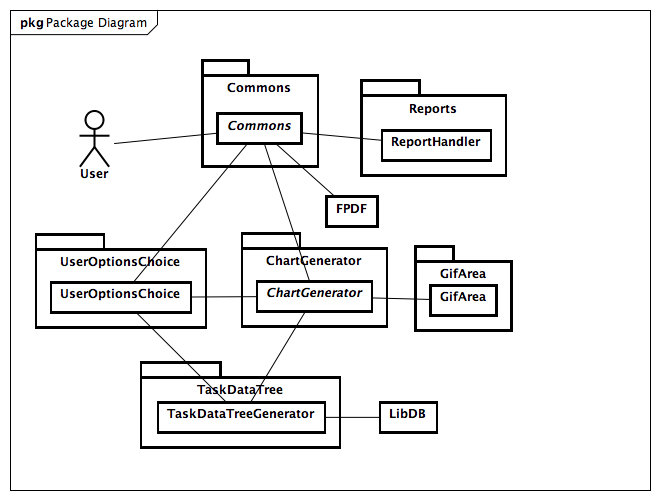
\includegraphics[width=\textwidth]{chart/PackageDiagram.png}
Il diagramma propone una visuale ad alto livello delle componenti principali del modulo.
\begin{itemize}
	\item Commons: questa componente \`e quella che controlla il flusso principale e si interfaccia direttamente con l'utente (la pressione dei pulsanti dell'interfaccia utente corrisponde a una chiamata di un metodo). Utilizza la componente ChartGenerator per generare i diagrammi richiesti e UserOptionsChoice per gestire la visualizzazione e l'acquisizione delle opzioni utente presenti nella form della pagina. Per includere il diagramma in un PDF \`e necessario che comunichi con la libreria FPDF, mentre per aggiungere i diagrammi al report deve utilizzare la componente Reports.
	\item ChartGenerator: questa componente si occupa della generazione dei diagrammi. \\
L'elaborazione grafica viene delegata alla componente GifArea, l'acquisizione dei dati a TaskDataTreeGenerator, e le opzioni utente vengono lette da UserOptionsChoice.
	\item TaskDataTreeGenerator: questa componente si occupa della generazione di una struttura dati contenente tutte le informazioni dei task di cui \`e composto il progetto. Si interfaccia con il database per il reperimento dei dati utilizzando la classe gi\`a presente in PMango \emph{DBQuery}. Le richieste di quali dati verranno richiesti al database dipendono dalle opzioni specificate in UserOptionsChoice.
	\item UserOptionsChoices: questa componente gestisce i campi di un array associativo che contiene le opzioni scelte dall'utente.
	\item GifArea: componente che contiene utilit\`a per l'elaborazione di immagini gif. Queste funzionalit\`a si collocano in un livello medio tra la generazione del diagramma completo e il disegno di segmenti e label.
	\item Reports: questo componente si occupa di aggiungere il diagramma prodotto nel report.
\end{itemize}
Le dipendenze esterne al modulo sono:
\begin{itemize}
	\item FPDF: la libreria per la generazione dei PDF 
	``lib/fpdf/fpdf.php''
	\item DBQuery: la classe per reperire le informazioni dal database 
	``classes/query.class.php''
\end{itemize}

\chapter{Class Diagrams}

\section{Commons}

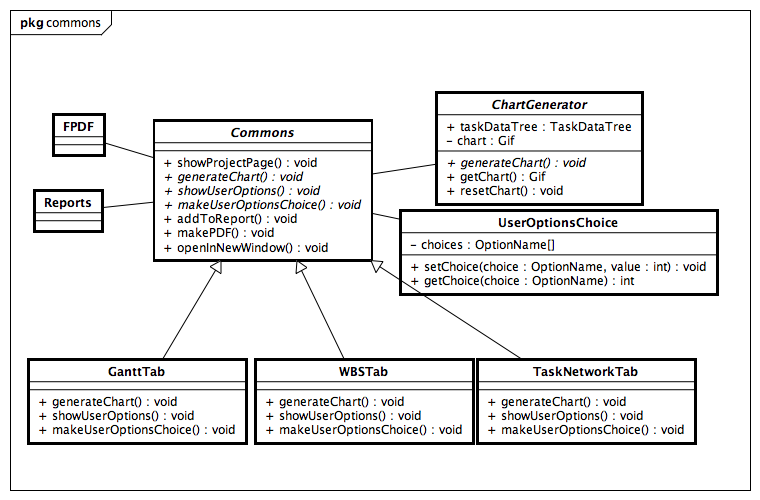
\includegraphics[width=\textwidth]{chart/Commons.png}
La classe Commons racchiude tutte le funzioni principali del modulo. Utilizza le classi
\begin{itemize}
	\item ChartGenerator
	\item UserOptionsChoice
	\item Reports
	\item FPDF (esterna al modulo e gi\`a utilizzata in PMango)
\end{itemize}
La classe \`e astratta a causa dei metodi astratti \emph{generateChart}, \emph{ShowUserOptions} e \emph{makeUserOptionsChoice} (che dovranno essere implementati nelle successive estensioni). In generale i metodi contenuti nella classe Commons sono quelli presentati nel documento dei casi d'uso, contentente una descrizione pi\`u approfondita dei
A seconda di quale tab viene caricato, pu\`o essere usata l'estensione di Commons corrispondente: 
\begin{itemize}
	\item GanttTab
	\item WBSTab
	\item TaskNetworkTab
\end{itemize}
che implementano la generazione del diagramma, la creazione della maschera delle user options e l'acquisizione delle scelte dei parametri.

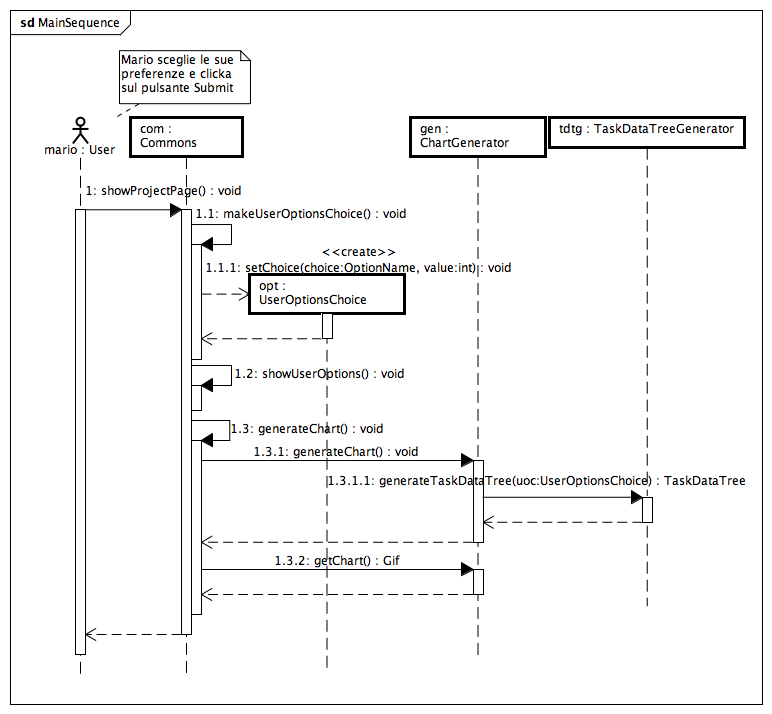
\includegraphics[width=\textwidth]{chart/MainSequence.png}

\section{Chart Generator}
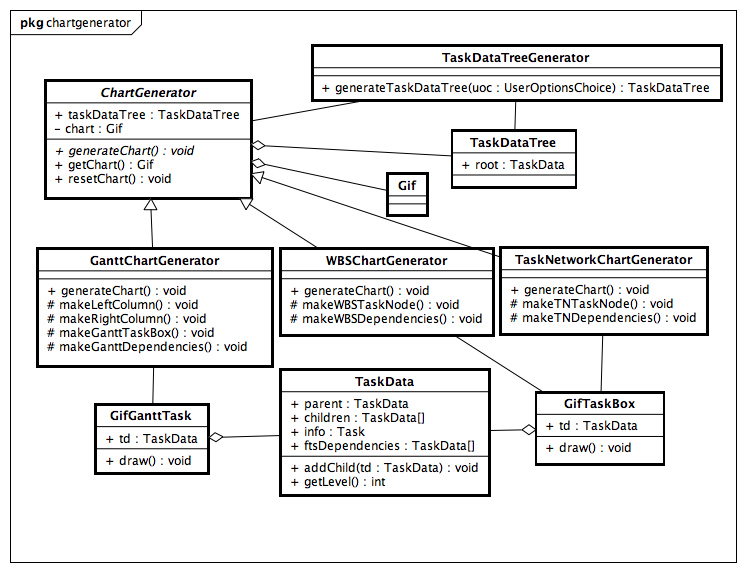
\includegraphics[width=\textwidth]{chart/ChartGenerator.png}

\section{Task Data}
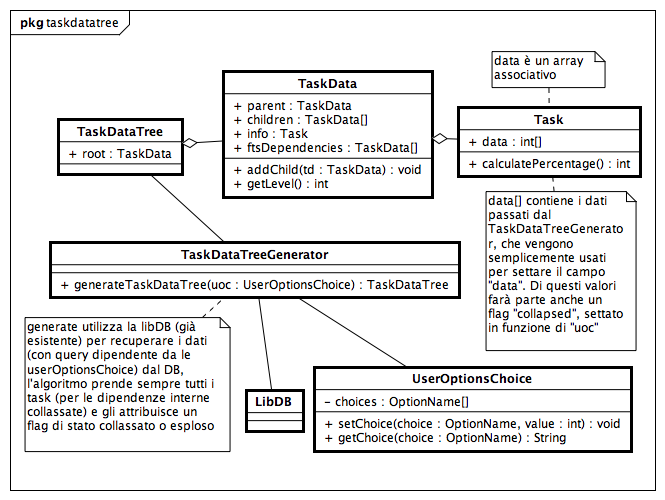
\includegraphics[width=\textwidth]{chart/TaskDataTree.png}

\section{Gif Area}
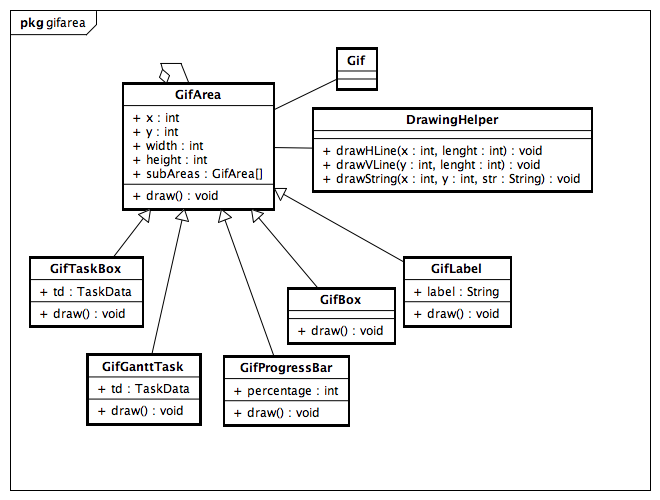
\includegraphics[width=\textwidth]{chart/GifArea.png}
La GifArea e i suo derivati realizzano il pattern \emph{composite} che si presta a portare ad un livello pi\`u alto la gestione della grafica, infatti qualunque cosa che sia una ``GifArea'' avr\`a la possibilità di essere stampata (tramite la funzione \emph{draw}) su una gif in un determinato punto $(x,y)$ occupando una certa area di dimensioni ``width'' e ``height''.
I componenti più base per maneggiare la grafica in questo contesto sono la ``GifLabel'' che \`e la rappresentazione grafica di un testo, la ``GifBox'' che \`e una rappresentazione grafica di un rettangolo, la ``GifProgressBar'' che che rappresenta una barra di completamento.
Anche i GifTaskBox sono una GifArea e sono composti da dei GifBox con al suo interno delle GifLabel, e da una GifProgressBar quando richiesta, e il draw del GifTaskBox far\`a il draw di tutti questi suoi componentini interni.
Una volta costruito l'albero dei taskdata sar\`a molto facile disegnare un GifTask da un taskdata.
Cos\`i si separano la visualizzazione dei taskbox dal problema del posizionamento e l'unione con le linee.

\section{User Options}
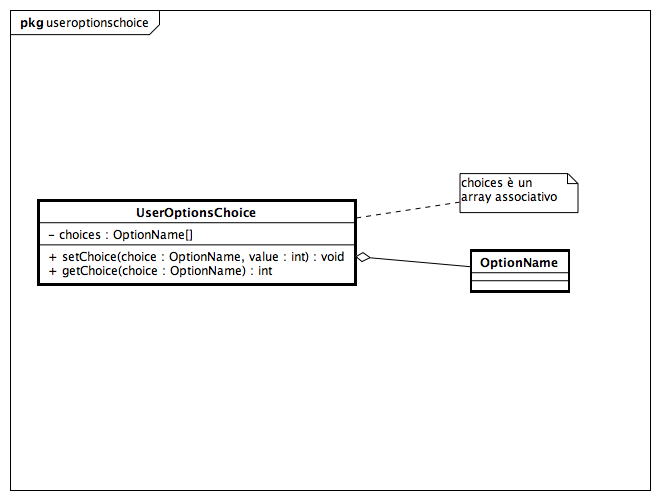
\includegraphics[width=\textwidth]{chart/UserOptionsChoice.png}
\begin{itemize}
	\item UserOptionsChoice: la classe che racchiude le scelte fatte dall'utente in un array associativo controllato dai metodi get e set.
	\item OptionName: un'enumerate che vincola l'accesso all'array associativo ai soli campi specificati. Questa contiene le seguenti voci (associate ai possibili valori che possono assumere):
	\begin{itemize}
		\item TaskNameOption: boolean		
		\item PlannedTimeFrameOption: boolean
		\item ActualTimeFrameOption: boolean
		\item PlannedDataOption: boolean
		\item ActualDataOption: boolean
		\item CompletitionBarOption: boolean
		\item AlertMarkUserOption: boolean
		\item WBSExplosionLevelUserOption: numeric
		\item WBSUserSpecificationUserLevel: boolean
		\item ReplicateArrowUserOption: boolean
		\item FindCriticalPathUserOption: boolean
		\item ResourcesDetailsOption: boolean
		\item CompleteDiagramUserOptions: boolean
		\item WBSTreeSpecification: LevelSpecification, UserCustomSpecification
		\item TimeGrain: HourlyGrain, DailyGrain, WeaklyGrain, MonthlyGrain, AnnualyGrain
		\item ImageDimensionUserOption: CustomDim, FitInWindowDim, OptionalDim, DefaultDim 
		\item TimeRangeUserOption: CustomRange, WholeProjectRange, FromStartRange, ToEndRange
	\end{itemize}
	La semantica di questi parametri \`e specificata nel domain model. Tutti i parametri boolean sono intesi $false$ se non presenti, \`e quindi necessario un doppio controllo per capire se \`e impostato il valore $true$: il controllo sulla presenza del campo ed eventualmente sul suo valore.
\end{itemize}

\section{Reports}
\end{document}
